% Created by tikzDevice version 0.12.3.1 on 2023-05-05 12:42:55
% !TEX encoding = UTF-8 Unicode
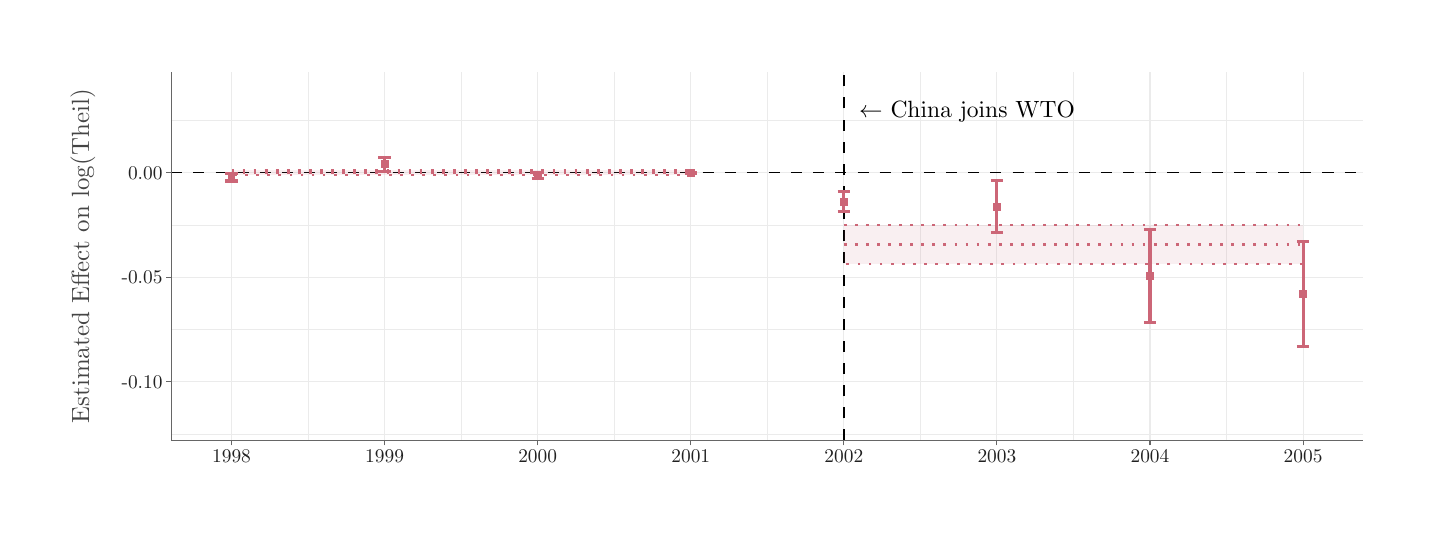
\begin{tikzpicture}[x=1pt,y=1pt]
\definecolor{fillColor}{RGB}{255,255,255}
\path[use as bounding box,fill=fillColor,fill opacity=0.00] (0,0) rectangle (498.66,174.53);
\begin{scope}
\path[clip] (  0.00,  0.00) rectangle (498.66,174.53);
\definecolor{fillColor}{RGB}{255,255,255}

\path[fill=fillColor] (  0.00,  0.00) rectangle (498.66,174.53);
\end{scope}
\begin{scope}
\path[clip] ( 51.87, 25.33) rectangle (482.66,158.53);
\definecolor{fillColor}{RGB}{255,255,255}

\path[fill=fillColor] ( 51.87, 25.33) rectangle (482.66,158.53);
\definecolor{drawColor}{gray}{0.92}

\path[draw=drawColor,line width= 0.2pt,line join=round] ( 51.87, 27.60) --
	(482.66, 27.60);

\path[draw=drawColor,line width= 0.2pt,line join=round] ( 51.87, 65.44) --
	(482.66, 65.44);

\path[draw=drawColor,line width= 0.2pt,line join=round] ( 51.87,103.28) --
	(482.66,103.28);

\path[draw=drawColor,line width= 0.2pt,line join=round] ( 51.87,141.13) --
	(482.66,141.13);

\path[draw=drawColor,line width= 0.2pt,line join=round] (101.32, 25.33) --
	(101.32,158.53);

\path[draw=drawColor,line width= 0.2pt,line join=round] (156.63, 25.33) --
	(156.63,158.53);

\path[draw=drawColor,line width= 0.2pt,line join=round] (211.95, 25.33) --
	(211.95,158.53);

\path[draw=drawColor,line width= 0.2pt,line join=round] (267.27, 25.33) --
	(267.27,158.53);

\path[draw=drawColor,line width= 0.2pt,line join=round] (322.58, 25.33) --
	(322.58,158.53);

\path[draw=drawColor,line width= 0.2pt,line join=round] (377.90, 25.33) --
	(377.90,158.53);

\path[draw=drawColor,line width= 0.2pt,line join=round] (433.21, 25.33) --
	(433.21,158.53);

\path[draw=drawColor,line width= 0.4pt,line join=round] ( 51.87, 46.52) --
	(482.66, 46.52);

\path[draw=drawColor,line width= 0.4pt,line join=round] ( 51.87, 84.36) --
	(482.66, 84.36);

\path[draw=drawColor,line width= 0.4pt,line join=round] ( 51.87,122.20) --
	(482.66,122.20);

\path[draw=drawColor,line width= 0.4pt,line join=round] ( 73.66, 25.33) --
	( 73.66,158.53);

\path[draw=drawColor,line width= 0.4pt,line join=round] (128.98, 25.33) --
	(128.98,158.53);

\path[draw=drawColor,line width= 0.4pt,line join=round] (184.29, 25.33) --
	(184.29,158.53);

\path[draw=drawColor,line width= 0.4pt,line join=round] (239.61, 25.33) --
	(239.61,158.53);

\path[draw=drawColor,line width= 0.4pt,line join=round] (294.92, 25.33) --
	(294.92,158.53);

\path[draw=drawColor,line width= 0.4pt,line join=round] (350.24, 25.33) --
	(350.24,158.53);

\path[draw=drawColor,line width= 0.4pt,line join=round] (405.55, 25.33) --
	(405.55,158.53);

\path[draw=drawColor,line width= 0.4pt,line join=round] (460.87, 25.33) --
	(460.87,158.53);
\definecolor{drawColor}{RGB}{0,0,0}

\path[draw=drawColor,line width= 0.6pt,dash pattern=on 4pt off 4pt ,line join=round] ( 51.87,122.20) -- (482.66,122.20);

\path[draw=drawColor,line width= 0.6pt,dash pattern=on 4pt off 4pt ,line join=round] (294.92, 25.33) -- (294.92,158.53);

\node[text=drawColor,anchor=base west,inner sep=0pt, outer sep=0pt, scale=  0.85] at (300.45,141.97) {$\leftarrow$ China joins WTO};
\definecolor{drawColor}{RGB}{204,102,119}

\path[draw=drawColor,line width= 1.1pt,line join=round] ( 71.45,121.97) --
	( 75.87,121.97);

\path[draw=drawColor,line width= 1.1pt,line join=round] ( 73.66,121.97) --
	( 73.66,119.13);

\path[draw=drawColor,line width= 1.1pt,line join=round] ( 71.45,119.13) --
	( 75.87,119.13);

\path[draw=drawColor,line width= 1.1pt,line join=round] (126.76,127.76) --
	(131.19,127.76);

\path[draw=drawColor,line width= 1.1pt,line join=round] (128.98,127.76) --
	(128.98,122.62);

\path[draw=drawColor,line width= 1.1pt,line join=round] (126.76,122.62) --
	(131.19,122.62);

\path[draw=drawColor,line width= 1.1pt,line join=round] (182.08,122.05) --
	(186.51,122.05);

\path[draw=drawColor,line width= 1.1pt,line join=round] (184.29,122.05) --
	(184.29,120.14);

\path[draw=drawColor,line width= 1.1pt,line join=round] (182.08,120.14) --
	(186.51,120.14);

\path[draw=drawColor,line width= 1.1pt,line join=round] (237.40,122.17) --
	(241.82,122.17);

\path[draw=drawColor,line width= 1.1pt,line join=round] (239.61,122.17) --
	(239.61,121.79);

\path[draw=drawColor,line width= 1.1pt,line join=round] (237.40,121.79) --
	(241.82,121.79);

\path[draw=drawColor,line width= 1.1pt,line join=round] (292.71,115.40) --
	(297.14,115.40);

\path[draw=drawColor,line width= 1.1pt,line join=round] (294.92,115.40) --
	(294.92,108.00);

\path[draw=drawColor,line width= 1.1pt,line join=round] (292.71,108.00) --
	(297.14,108.00);

\path[draw=drawColor,line width= 1.1pt,line join=round] (348.03,119.23) --
	(352.45,119.23);

\path[draw=drawColor,line width= 1.1pt,line join=round] (350.24,119.23) --
	(350.24,100.48);

\path[draw=drawColor,line width= 1.1pt,line join=round] (348.03,100.48) --
	(352.45,100.48);

\path[draw=drawColor,line width= 1.1pt,line join=round] (403.34,101.68) --
	(407.77,101.68);

\path[draw=drawColor,line width= 1.1pt,line join=round] (405.55,101.68) --
	(405.55, 68.01);

\path[draw=drawColor,line width= 1.1pt,line join=round] (403.34, 68.01) --
	(407.77, 68.01);

\path[draw=drawColor,line width= 1.1pt,line join=round] (458.66, 97.11) --
	(463.08, 97.11);

\path[draw=drawColor,line width= 1.1pt,line join=round] (460.87, 97.11) --
	(460.87, 59.42);

\path[draw=drawColor,line width= 1.1pt,line join=round] (458.66, 59.42) --
	(463.08, 59.42);
\definecolor{fillColor}{RGB}{204,102,119}

\path[fill=fillColor] ( 72.24,119.12) --
	( 75.09,119.12) --
	( 75.09,121.98) --
	( 72.24,121.98) --
	cycle;

\path[fill=fillColor] (127.55,123.77) --
	(130.40,123.77) --
	(130.40,126.62) --
	(127.55,126.62) --
	cycle;

\path[fill=fillColor] (182.87,119.67) --
	(185.72,119.67) --
	(185.72,122.52) --
	(182.87,122.52) --
	cycle;

\path[fill=fillColor] (238.18,120.55) --
	(241.03,120.55) --
	(241.03,123.41) --
	(238.18,123.41) --
	cycle;

\path[fill=fillColor] (293.50,110.27) --
	(296.35,110.27) --
	(296.35,113.12) --
	(293.50,113.12) --
	cycle;

\path[fill=fillColor] (348.81,108.43) --
	(351.66,108.43) --
	(351.66,111.28) --
	(348.81,111.28) --
	cycle;

\path[fill=fillColor] (404.13, 83.42) --
	(406.98, 83.42) --
	(406.98, 86.27) --
	(404.13, 86.27) --
	cycle;

\path[fill=fillColor] (459.44, 76.84) --
	(462.30, 76.84) --
	(462.30, 79.69) --
	(459.44, 79.69) --
	cycle;
\definecolor{fillColor}{RGB}{204,102,119}

\path[fill=fillColor,fill opacity=0.10] (294.92,103.14) --
	(460.87,103.14) --
	(460.87, 89.19) --
	(294.92, 89.19) --
	cycle;

\path[draw=drawColor,line width= 0.6pt,dash pattern=on 1pt off 3pt ,line join=round] (294.92,103.14) --
	(460.87,103.14);

\path[draw=drawColor,line width= 0.6pt,dash pattern=on 1pt off 3pt ,line join=round] (460.87, 89.19) --
	(294.92, 89.19);

\path[fill=fillColor,fill opacity=0.10] ( 73.66,123.00) --
	(239.61,123.00) --
	(239.61,121.41) --
	( 73.66,121.41) --
	cycle;

\path[draw=drawColor,line width= 0.6pt,dash pattern=on 1pt off 3pt ,line join=round] ( 73.66,123.00) --
	(239.61,123.00);

\path[draw=drawColor,line width= 0.6pt,dash pattern=on 1pt off 3pt ,line join=round] (239.61,121.41) --
	( 73.66,121.41);

\path[draw=drawColor,line width= 1.1pt,dash pattern=on 1pt off 3pt ,line join=round] (294.92, 96.16) --
	(460.87, 96.16);

\path[draw=drawColor,line width= 1.1pt,dash pattern=on 1pt off 3pt ,line join=round] ( 73.66,122.20) --
	(239.61,122.20);
\end{scope}
\begin{scope}
\path[clip] (  0.00,  0.00) rectangle (498.66,174.53);
\definecolor{drawColor}{gray}{0.40}

\path[draw=drawColor,line width= 0.4pt,line join=round] ( 51.87, 25.33) --
	( 51.87,158.53);
\end{scope}
\begin{scope}
\path[clip] (  0.00,  0.00) rectangle (498.66,174.53);
\definecolor{drawColor}{gray}{0.13}

\node[text=drawColor,anchor=base east,inner sep=0pt, outer sep=0pt, scale=  0.70] at ( 48.72, 44.11) {-0.10};

\node[text=drawColor,anchor=base east,inner sep=0pt, outer sep=0pt, scale=  0.70] at ( 48.72, 81.95) {-0.05};

\node[text=drawColor,anchor=base east,inner sep=0pt, outer sep=0pt, scale=  0.70] at ( 48.72,119.79) {0.00};
\end{scope}
\begin{scope}
\path[clip] (  0.00,  0.00) rectangle (498.66,174.53);
\definecolor{drawColor}{gray}{0.40}

\path[draw=drawColor,line width= 0.4pt,line join=round] ( 50.12, 46.52) --
	( 51.87, 46.52);

\path[draw=drawColor,line width= 0.4pt,line join=round] ( 50.12, 84.36) --
	( 51.87, 84.36);

\path[draw=drawColor,line width= 0.4pt,line join=round] ( 50.12,122.20) --
	( 51.87,122.20);
\end{scope}
\begin{scope}
\path[clip] (  0.00,  0.00) rectangle (498.66,174.53);
\definecolor{drawColor}{gray}{0.40}

\path[draw=drawColor,line width= 0.4pt,line join=round] ( 51.87, 25.33) --
	(482.66, 25.33);
\end{scope}
\begin{scope}
\path[clip] (  0.00,  0.00) rectangle (498.66,174.53);
\definecolor{drawColor}{gray}{0.40}

\path[draw=drawColor,line width= 0.4pt,line join=round] ( 73.66, 23.58) --
	( 73.66, 25.33);

\path[draw=drawColor,line width= 0.4pt,line join=round] (128.98, 23.58) --
	(128.98, 25.33);

\path[draw=drawColor,line width= 0.4pt,line join=round] (184.29, 23.58) --
	(184.29, 25.33);

\path[draw=drawColor,line width= 0.4pt,line join=round] (239.61, 23.58) --
	(239.61, 25.33);

\path[draw=drawColor,line width= 0.4pt,line join=round] (294.92, 23.58) --
	(294.92, 25.33);

\path[draw=drawColor,line width= 0.4pt,line join=round] (350.24, 23.58) --
	(350.24, 25.33);

\path[draw=drawColor,line width= 0.4pt,line join=round] (405.55, 23.58) --
	(405.55, 25.33);

\path[draw=drawColor,line width= 0.4pt,line join=round] (460.87, 23.58) --
	(460.87, 25.33);
\end{scope}
\begin{scope}
\path[clip] (  0.00,  0.00) rectangle (498.66,174.53);
\definecolor{drawColor}{gray}{0.13}

\node[text=drawColor,anchor=base,inner sep=0pt, outer sep=0pt, scale=  0.70] at ( 73.66, 17.36) {1998};

\node[text=drawColor,anchor=base,inner sep=0pt, outer sep=0pt, scale=  0.70] at (128.98, 17.36) {1999};

\node[text=drawColor,anchor=base,inner sep=0pt, outer sep=0pt, scale=  0.70] at (184.29, 17.36) {2000};

\node[text=drawColor,anchor=base,inner sep=0pt, outer sep=0pt, scale=  0.70] at (239.61, 17.36) {2001};

\node[text=drawColor,anchor=base,inner sep=0pt, outer sep=0pt, scale=  0.70] at (294.92, 17.36) {2002};

\node[text=drawColor,anchor=base,inner sep=0pt, outer sep=0pt, scale=  0.70] at (350.24, 17.36) {2003};

\node[text=drawColor,anchor=base,inner sep=0pt, outer sep=0pt, scale=  0.70] at (405.55, 17.36) {2004};

\node[text=drawColor,anchor=base,inner sep=0pt, outer sep=0pt, scale=  0.70] at (460.87, 17.36) {2005};
\end{scope}
\begin{scope}
\path[clip] (  0.00,  0.00) rectangle (498.66,174.53);
\definecolor{drawColor}{gray}{0.27}

\node[text=drawColor,rotate= 90.00,anchor=base,inner sep=0pt, outer sep=0pt, scale=  0.90] at ( 22.20, 91.93) {Estimated Effect on $\log($Theil$)$};
\end{scope}
\end{tikzpicture}
